\section{Cubic vs BBR}

Sia Cubic (App. A) che BBR, si servono di uno stato iniziale, quali lo Slow Start e lo Startup (rispettivamente), per scovare rapidamente il limite superiore del delivery rate. \bigskip

Tuttavia, hanno un intento differente, essendo due approcci al controllo di congestione diversi. \bigskip

Il Cubic cerca il limite superiore per fissare la soglia di passaggio dallo Slow Start, al Congestion Avoidance. In cui semplicemente, continuerà ad aumentare il sending rate, ma in modo più lento. Questo finchè non raggiungerà il punto in cui scadrà un timeout, o il bottleneck buffer sarà saturo. Condizione in cui si verificheranno delle perdite. \bigskip

Il BBR invece, raggiunto il limite del delivery rate, con la consapevolezza di esser andato un pò oltre (il target point) e di aver generato delle code, passa in Drain per scaricarle.
Quindi arriva in ProbeBW con le condizioni giuste e necessarie ad operare regolarmente al massimo tasso, ed ai minimi ritardi. \bigskip

Possiamo infatti sottolineare la loro evidente differenza nella gestione dell'RTT, con il seguente scenario:

\begin{figure}[H]

\center
\caption{First second of a 10Mbps, 40ms BBR flow}
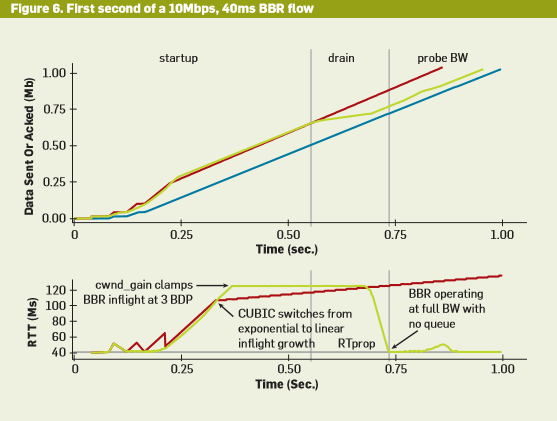
\includegraphics[scale=1.1]{chapters/4_application/img/start_cubic_bbr}
\caption*{Figura tratta da \cite[p.~63]{Cardwell:2017:BCC:3042068.3009824}}

\end{figure}

L'ambito operativo di Cubic è sicuramente quello peggiore, in quanto avremo dei livelli alternati di RTT, tra il 70\% ed il 100\% (con 0\% intendiamo la condizione in cui RTT $ \simeq $ RTprop), ed un delivery rate si al massimo, ma dimezzato ogni volta in corrispondenza di una perdita (o abbattuto ad un timeout):

\begin{figure}[H]

\center
\caption{First eight seconds of a 10Mbps, 40ms cubic and BBR flow}
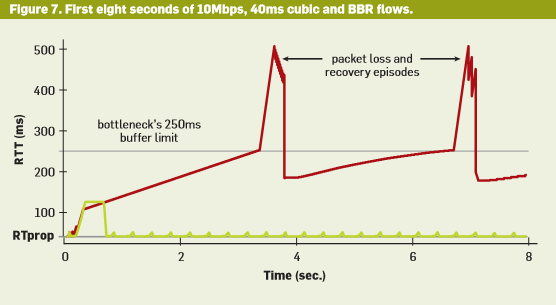
\includegraphics[scale=1.1]{chapters/4_application/img/rtt_cubic_bbr}
\caption*{Figura tratta da \cite[p.~64]{Cardwell:2017:BCC:3042068.3009824}}

\end{figure}

Bisogna però prendere atto di una cosa, ovvero che Cubic a differenza del BBR non dispone di un network path model. Quindi non è possibile contenere l'RTT se non lo si traccia nel tempo, e se non è quest'ultimo a determinare il valore dei parametri di controllo della soluzione.

\section{Fairness tra flussi BBR}

Tra flussi BBR concorrenti, il livello di fairness raggiunto, testimoniato anche da appositi esperimenti, è molto soddisfacente. \bigskip

Ecco infatti un caso d'esempio di 5 flussi concorrenti, che condividono un bottleneck link da 100 Mbps, ed un RTT da 10 ms:

\begin{figure}[H]

\center
\caption{Throughput of five BBR flows sharing a bottleneck}
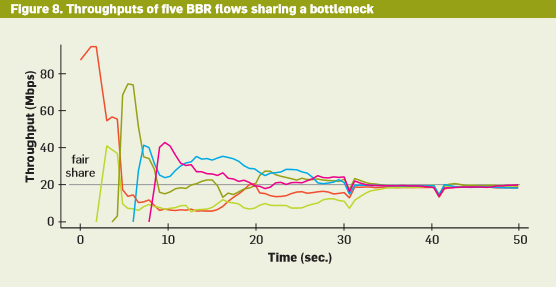
\includegraphics[scale=1.1]{chapters/4_application/img/fairness_bbr}
\caption*{Figura tratta da \cite[p.~64]{Cardwell:2017:BCC:3042068.3009824}}

\end{figure}

Nella figura viene presentato uno scenario abbastanza generale, in cui i flussi BBR non nascono tutti nello stesso istante. \bigskip

Ciò che ci aspettiamo accada è semplice. Nello stato di ProbeBW i flussi al di sopra del fair share scopriranno un calo del bottleneck rate, quindi si accorgeranno della perdita di banda, riconfigurando poi il loro pacing rate. \bigskip

Andando poi avanti, quando (di nuovo) un flusso al di sopra del fair share - che dunque sta generando un maggior traffico - entrerà in ProbeRTT, svuoterà considerevolmente il bottleneck buffer. Ciò porterà ad un aggiornamento dell'RTprop degli altri flussi concorrenti. \bigskip

Alla lunga, il tutto porta a sincronizzare l'entrata nello stato di ProbeRTT di tutti i flussi. Così tutti portranno stimare il reale valore dell'RTprop, così come del bottleneck rate.

\section{Fairness tra flussi loss-based e BBR}

In questo caso, è abbastanza (purtroppo) prevedibile che allo stato attuale delle cose, sia difficile raggiungere una suddivisione equa della banda. \bigskip

Fondamentalmente, un flusso loss-based presenta un andamento del throughput pressochè a dente di sega:

\begin{figure}[H]

\center
\caption{TCP loss-based evoluzione del throughput}
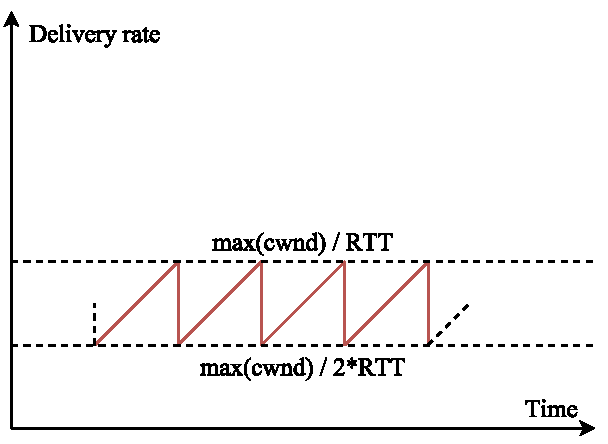
\includegraphics[scale=0.8]{chapters/4_application/img/tcp_reno}

\end{figure}

Allora ci aspetteremo che un flusso BBR abbia maggiore banda nelle fasi di low-throughput del flusso loss, mentre questi diminuisca quando quest'ultimo arriva al suo massimo (le sue reali possibilità). Tuttavia, un flusso loss, ad esempio come Reno, raggiunge il massimo in corrispondenza di un evento di perdita, per cui non manterrà a lungo tale livello. \bigskip

Per la consultazione di appositi esperimenti si veda \cite{ietf:ietf-98-bbr-slides}. 

\section{Rete Google B4}

B4 è una rete proprietaria ad estensione geografica, dalle alte performance, di Google. \bigskip

Nel 2015, quando BBR non era più solo una teoria, ma una idea concreta, si diede inizio ad una transizione verso quest'ultimo. Così nel 2016, Cubic è stato completamente sostituito dal BBR, che non essendo un approccio loss-based, ha portato un notevole incremento delle prestazioni. \bigskip

Il primo artefatto d'analisi mette a rapporto il throughput raggiunto con BBR rispetto quello raggiunto con Cubic:

\begin{figure}[H]

\center
\caption{BBR vs CUBIC relative throughput improvement}
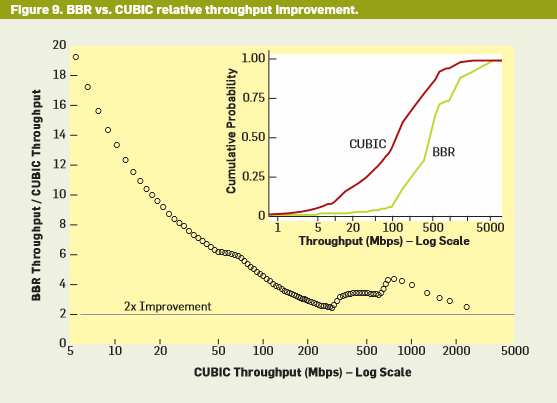
\includegraphics[scale=1]{chapters/4_application/img/bbr_vs_cubic_1}
\caption*{Figura tratta da \cite[p.~64]{Cardwell:2017:BCC:3042068.3009824}}

\end{figure}

Tali dati, raccolti da varie sonde disposte in vari punti della rete B4, mettono in evidenza un incremento prestazionale che va dal 2x al 25x. In realtà, l'incremento del BBR è mascherato dal limite imposto ai buffer di ricezione TCP (8 MB). \bigskip

Alzando tale limite, è stato ottenuto su un path tra Europa e USA, un throughput di 2 Gbps, contro i 15 Mbps di Cubic. Parliamo di un incremento: 133x. \bigskip

Nel grafico vengono anche messe a confronto le distribuzioni di probabilità cumulative. Da esso possiamo notare (qualitativamente) che:

\begin{table}[H]

\centering
\caption{Throughput CDF}	

\begin{tabular}{ccc}

\toprule
 & BBR & Cubic \\
\midrule
P(thput < 1) & $ \simeq $ 0 & $ \simeq $ 0 \\
\midrule
P(thput < 20) & $ \simeq $ 0 & 0.19  \\
\midrule
P(thput < 100) & 0.06 & 0.5 \\
\midrule
P(thput < 500) & 0.62 & 0.87  \\
\midrule
P(thput < 5000) & 1 & 1  \\
\bottomrule

\end{tabular}
\end{table}

Il secondo artefatto mette a confronto il throughput utile sostenibile in funzione del loss-rate:

\begin{figure}[H]

\center
\caption{BBR vs CUBIC goodput under loss}
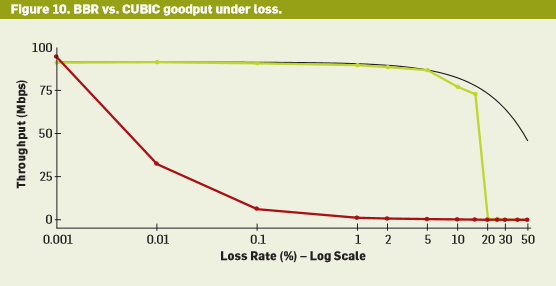
\includegraphics[scale=1]{chapters/4_application/img/bbr_vs_cubic_loss_rate}
\caption*{Figura tratta da \cite[p.~65]{Cardwell:2017:BCC:3042068.3009824}}

\end{figure}

Ricordando che un loss-rate ragionevole è circa dell'1\%, e notando che il BBR perde performance tra 5\% ed 20\%, questo è un ottimo miglioramento.

%\section{Youtube}